% Updated in May 2014 by Hideo Saito
% Updated in March 2012 by Yasuyuki Matsushita
% Updated in April 2002 by Antje Endemann, ...., and in March 2010 by Reinhard Klette
% Based on CVPR 07 and LNCS style, with modifications by DAF, AZ and elle 2008, AA 2010, ACCV 2010

\documentclass[runningheads]{llncs}
\usepackage{graphicx}
\usepackage{amsmath,amssymb} % define this before the line numbering.
\usepackage{ruler}
\usepackage{color}

\usepackage{epstopdf}
\usepackage{times}
\usepackage{epsfig}
\usepackage{graphicx}
\usepackage{url}
\usepackage{bm}

%===========================================================
\begin{document}
\pagestyle{headings}
\mainmatter

%\psdraft


\def\ACCV14SubNumber{215}  % Insert your submission number here

%===========================================================
\title{Clouds in The Cloud} % Replace with your title
\titlerunning{ACCV-14 submission ID \ACCV14SubNumber}
\authorrunning{ACCV-14 submission ID \ACCV14SubNumber}

\author{Anonymous ACCV 2014 submission}
\institute{Paper ID \ACCV14SubNumber}

\maketitle

%===========================================================
\begin{abstract}
Light-field imaging can be scaled up to continental size, to map the Earth's atmosphere in 3D. Multiview spaceborne instruments suffer low spatio-temporal and angular resolution, and are extremely expensive and unscalable. We develop lightfield imaging of the sky, by a scalable network of wide-angle cameras  looking upwards, which upload their data to the cloud. This new type of imaging-system poses {\em new computational vision and photography problems}, some of which generalize prior monocular tasks. These include radiometric self-calibration across a network, overcoming flare by a network, and background estimation. On the other hand, network redundancy offers {\em solutions} to these problems, which we derive. Based on such solutions, the light-field network enables unprecedented ways to measure nature. We demonstrate this experimentally by 3D recovery of clouds, in high spatio-temporal resolution. It is achieved by space carving of the volumetric distribution of semi-transparent clouds. This sensing approach can complement satellite imagery, be useful to aviation meteorology and study of birds. The radiometric capabilities can make aerosol tomography realizable, and give new, powerful tools to atmospheric scientists.

\end{abstract}

%===========================================================
\section{Introduction}

Following the introduction of plenotic imaging to computer vision~\cite{Adelson1992}, light-field imaging~\cite{Basha2012,bishop,horstmeyer,Ng1948,kim} has had a significant impact on sensing. This modality samples the radiance distribution in location and direction. It has so far been used mainly in small-scale setups. However, it can be scaled up to continental size, to map the Earth's atmosphere in 3D. Sampling the atmospheric radiance spatio-angularly is achieved by a few spaceborne and airborne instruments, including the Multiangle Imaging SpectroRadiometer (MISR)~\cite{diner,Diner1998}, the Airborne Multiangle SpectroPolarimetric Imager (AirMSPI)~\cite{dinerDavis07,dinerDavis10} and POLDER~\cite{baxter,breon,vanMol}.
However, these imaging architectures suffer from several drawbacks. They have crude resolution spatially (effectively several kilometers per pixel), angularly  ($\approx 7$ angles per view), and temporally (orbit takes several days to return to the same terrestrial spot). Furthermore, spaceborne instruments are extremely expensive and unscalable. Hence, in this work we develop a counter approach: the atmospheric lightfield is captured  from below, by wide-angle cameras looking upwards. Moreover, instead of expensive one-off instruments, our approach is a {\em scalable sensor network} that captures images simultaneously over a very large area, densely.

Creating and exploiting such a light-field imaging-network poses several requirements: low-cost units,
communications, and {\em tailored computational photography algorithms}. The first two requirements are met  thanks to cellular-network infrastructure, cellular-based low-cost cameras and {\em cloud computing} services. Hence, we can deploy solar-powered cameras at will, nearly anywhere. By wireless, they upload their sky-images to the ``cloud'', from which the light-field data can be analyzed. However, this new type of imaging-system gives rise to new problems and algorithms, part of which we deal with in this paper. In a sense, the network generalizes some computer vision problems that had been posed for monocular setups a decade ago. On the other hand, network redundancy offers {\em solutions} to these problems.

The computational photography problems include radiometric self-calibration across a network of cameras, background estimation, and overcoming saturation and flare by a network. Consequently, the light-field network enables unprecedented 3D imaging of clouds, in high spatio-temporal resolution.  We demonstrate the approach using real field experiments. As a result, we believe this approach can complement multi-angular satellite cloud imagery, perhaps make aerosol tomography~\cite{Aides:13} realizable, and offer new capabilities to study weather phenomena and birds.



%%%%%%%%%%%%%%%%%%%%%%%%%%%%%%%%%%%%%%%%%%%%%%%%%%%%%%%%%%%%%%
\section{Background}
\label{sec:theory}


%%%%%%%%%%%%%%%%%%%%%%%%%%%%%%%%%%%%%%%%%%%%%%%%%%%%%%%%%%%%%%
\subsection{Monocular radiometric self-calibration}
\label{sec:Signelradio}

A large network should use low-cost camera units. Such cameras often have spatial and temporal radiometric inconsistencies. For a single camera, consistent readouts can be obtained in the field by self-calibration. The strongest methods rely on redundant images, taken at modulated settings. In particular, images taken during slow panning yield spatial non-uniformity correction (NUC) of offset and gain (e.g., by vignetting~\cite{LitvinovCVPR05,Kang2000}). For example, spatial gain is often modeled by a function $M({\bf x})$, where \mbox{${\bf x}=(x,y)$} is a camera pixel. Thus the image pixel irradiance at time $t$ is
\begin{equation}
 \tilde{I}_t({\bf x}) = M({\bf x})I_t(O) \;,
 \label{eq:tilde_I}
\end{equation}
where $I_t(O)$ is the pixel irradiance when $M=1$, for observed object $O$. Let the camera be panned, so that the object $O$ projects to pixel ${\bf x}'$ in time $t'$.
{\em Correspondence} is established between the two pixels, by image alignment. This yields a redundant measurement $\tilde{I}_t'({\bf x}') = M({\bf x}')I_t'(O)$. Assuming brightness constancy, $I_t(O)=I_t'(O)$, the two measurements yield a linear constraint
\begin{equation}
 \log M({\bf x})- \log M({\bf x}')=\log \tilde{I}_t({\bf x})-\log \tilde{I}_t'({\bf x}').
 \label{eq:logM}
\end{equation}
Aggregating such constraints over different pixels and frames recovers $M({\bf x})$, up to a global exponential ambiguity. This recovery makes pixel readout spatially consistent. Similar formulations exist for an additive offset. In Sec.~\ref{sec:mutiradio} we expand this principle to a camera-array.



%%%%%%%%%%%%%%%%%%%%%%%%%%%%%%%%%%%%%%%%%%%%%%%%%%%%%%%%%%%%%%
\subsection{Avoiding Blooming, Lens-Flare in a Single Camera}
\label{sec:Signelflare}

In a wide-angle sky-viewing camera, sun-rays are liable to frequently shine directly into the lens. This can create blooming. Moreover, sun-rays create an additive, spatially varying lens-flare. Reducing lens flare was suggested~\cite{Koreban2009,Raskar2008,Talvala2007,Rouf2011}, using either a specialized detector array for nearby objects, or by camera rotation during imaging of a static scene. Both approaches complicate the need for simple, low-cost units and operation.
%Third, direct sunlight repeatedly entering the camera chamber and hitting pixels may damage the camera after a while.

Consequently, sky-observing wide-field cameras often have a {\em dynamic sun blocker}. It is essentially an opaque object raised above the camera optics, blocking the Sun from view. There are various configurations, but all of them {\em move}, as the Sun direction changes during the day and across the year. Motorized solutions~\cite{Pust2008} that need to work year-around significantly complicate such camera units, making them very expensive. In Sec.~\ref{sec:mutiSun} explains that a large camera network inherently bypasses the problem, without a need to constantly move a Sun blocker.




%%%%%%%%%%%%%%%%%%%%%%%%%%%%%%%%%%%%%%%%%%%%%%%%%%%%%%%%%%%%%%
\subsection{Current 3D Cloud Mapping}
\label{sec:current3D}

Existing sky-imaging systems used for research and operational meterology\footnote{There are also ground viewing webcams that happen to see sky parts~\cite{bradley,jacobs14cloudmap} and weather cameras
that are too sparse to be integrated for recovery.} are few, relying on high quality cameras and other parts~\cite{allmen,angeo-27-953-2009,cazorla,long,Seiz,kassianov}. Due to their complexity and costs, they were only used to estimate {\em cloud-base} over narrow regions right above a narrow-baseline camera pair. Satellite-based estimation of 3D {\em cloud-tops} has been proposed by MISR~\cite{Seiz2006}. It takes several minutes for MISR to capture multiple viewpoints of a region, during which the clouds generally move. Weather radars sense {\em raindrops}, which are much larger than cloud-drops and ice crystals. Hence radar does not sense clouds that do not produce rain.




%%%%%%%%%%%%%%%%%%%%%%%%%%%%%%%%%%%%%%%%%%%%%%%%%%%%%%%%%%%%%%
\section{Self-Calibration in a Camera Network}
\label{sec:muticalib}

Even in high grade equipment, there are generally radiometric inconsistencies between cameras. Hence, the same distant object has slightly different intensity readouts for different cameras. This problem may exacerbate in low-cost cameras, which have loose quality control. A large light-field network would need to use many such cameras. Estimating and compensating for inter-camera differences is helpful for subsequent computer vision algorithms. Consistency is necessary for radiometric-based tasks, such as tomography~\cite{Aides:13}.
%However, it also assists non-radiometric, higher level tasks. For example, consider cloud segmentation. Segmentation (which may rely on image-value thresholds) has to be as consistent as possible across different viewpoints, otherwise contradictions may arise.
 Similarly to Sec.~\ref{sec:Signelradio}, the solution relies on redundant measurement at {\em corresponding} points.   For correspondence, geometric calibration~\cite{Seiz2002} is a first necessity, which is treated in Sec.~\ref{sec:geometry}.


%%%%%%%%%%%%%%%%%%%%%%%%%%%%%%%%%%%%%%%%%%%%%%%%%%%%%%%%%%%%%%
\subsection{Geometric calibration}
\label{sec:geometry}

The cameras are deployed in the field. The location vector ${\bf l}_c$
of each camera $c$ is known by GPS, and the internal parameters $\Psi_c$ are pre-calibrated in the lab. However, the orientation (yaw, pitch and roll angle vector ${\bf \Theta}_c$) is loosely set, as the camera is placed in the field. The orientation is calibrated by automatically detecting and tracking extra-terrestrial (XT) objects (Moon, planets, Sun)~\cite{Seiz2002,lalonde}, across night or day\footnote{In~\cite{Seiz2002}, calibration relied on manual tracking of a special flight and long exposures at night.} in the hemispherical field of view.  Using astronomical charts per time $t$ and ${\bf l}_c$, an XT object is known to be at angle vector (zenith, azimuth) ${\bm \theta}^{\rm XT}(t)$ relative to a global coordinate system. Given camera orientation ${\bf \Theta}_c$, a ray from ${\bm \theta}^{\rm XT}(t)$ should project to pixel:
\begin{equation}
{\bf x}^{\rm XT}_{\rm model}(t) = {\Pi}({\bm \theta}^{\rm XT}(t);{\bf \Theta}_c,\Psi_c)
\;,
 \label{eq:xt}
\end{equation}
where ${\Pi}$ denotes projection (converting ray angles to image pixels).
The actual measured pixel ${\bf x}^{\rm XT}_{\rm measured}(t)$ has uncertainty, due to the finite angular size of the XT object and blooming. However, during the course of a day or night, the number of frames
  $N^{\rm frames}$ is ${\cal O}(100)$, leading to a simple optimization formulation:
\begin{equation}
 \hat{\bf \Theta}_c=\arg\min_{{\bf \Theta}_c}
 \sum_{t=1}^{N^{\rm frames}}
 \|{\Pi}({\bm \theta}^{\rm XT}(t);{\bf \Theta}_c,\Psi_c) - {\bf x}^{\rm XT}_{\rm measured}(t)\|^2
\;.
 \label{eq:hatThetac}
\end{equation}
We solved it using exhaustive search or gradient descent from null initialization, with the same results. The orientation calibration is illustrated in Fig.~\ref{fig:sunmotion}.
\begin{figure}[t!]
\begin{center}
   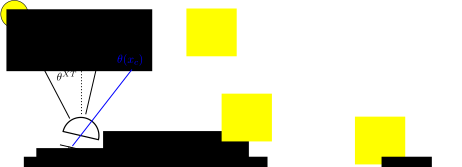
\includegraphics[width=0.7\linewidth]{figures/sun_moon.eps}
\end{center}
   \vspace{-0.6cm}
   \caption{(a) To estimate the camera yaw-pitch-roll angle vector ${\bf \Theta}_c$, we rely on
   image locations of extra-terrestrial objects, whose direction vector ${\bm \theta}^{\rm XT}(t)$
   is known for all time $t$. (b) Photo-montage of night sky images. It shows the Moon at different times, the expected trajectory based on the estimated ${\bf \Theta}_c$, and a close-up on the corresponding sampled images of Jupiter. (c) Photo-montage of the daylight sky. It shows the Sun at different hours, the expected trajectory based on the estimated ${\bf \Theta}_c$ and lens-flares.
   }
\label{fig:sunmotion}
\end{figure}


Based on $\hat{\bf \Theta}_c$, all captured images $\tilde I_{c,t}(\bf x)$ taken by camera $c$ are aligned to the global coordinate system. Any image pixel ${\bf x}$ of camera $c$ is backprojected to a ray at direction vector ${\bm \theta}$ in the global system, given by
\begin{equation}
 {\bm \theta}({\bf x})={\Pi}^{-1}({\bf x};\hat{\bf{\Theta}}_c,\Psi_c)
  \;.
 \label{eq:thetac}
\end{equation}
The sampled light-field is the radiance measured per location, direction and time, thus given by
$\tilde I_t[{\bf l}_c,{\bm \theta}(\bf x)]$.

 %%%%%%%%%%%%%%%%%%%%%%%%%%%%%%%%%%%%%%%%%%%%%%%%%%%%%%%%%%%%%%
\section{Some Details About The Experimental Setup}
\label{sec:set}

Before proceeding with mathematical problems and solutions, we describe  a small experimental network, which we built to test the hypotheses. To show that it can work with very low-cost  camera nodes (units), each of the 5 units was built from basic components, and coarse alignment tolerances. Its core is a Raspberry-Pi computer used in DIY electronics, and a 5MP Raspberry-Pi camera. In this camera, the gain, response and white-balance can be fixed, avoiding temporal radiometric variations. We cut-off its OEM lens, and manually mounted a small fisheye lens. Due to this coarse lens-to-chip alignment, {\em each camera has a different peripheral dead-region}, creating a missing part in the hemispheric view-field and vignetting distinct to each camera. As derived below, a {\em {\em network} as-a-whole} can inherently overcome these issues. Every 30 seconds, synchronously, all units automatically transmit image data using the cellular network to the internet (cloud-service). Each unit is solar powered (Fig.~\ref{fig:photomotion}).
The units were placed on several rooftops and ran for weeks, capturing 70GB of sky imagery.
%\begin{figure}[t!]
%\begin{center}
%   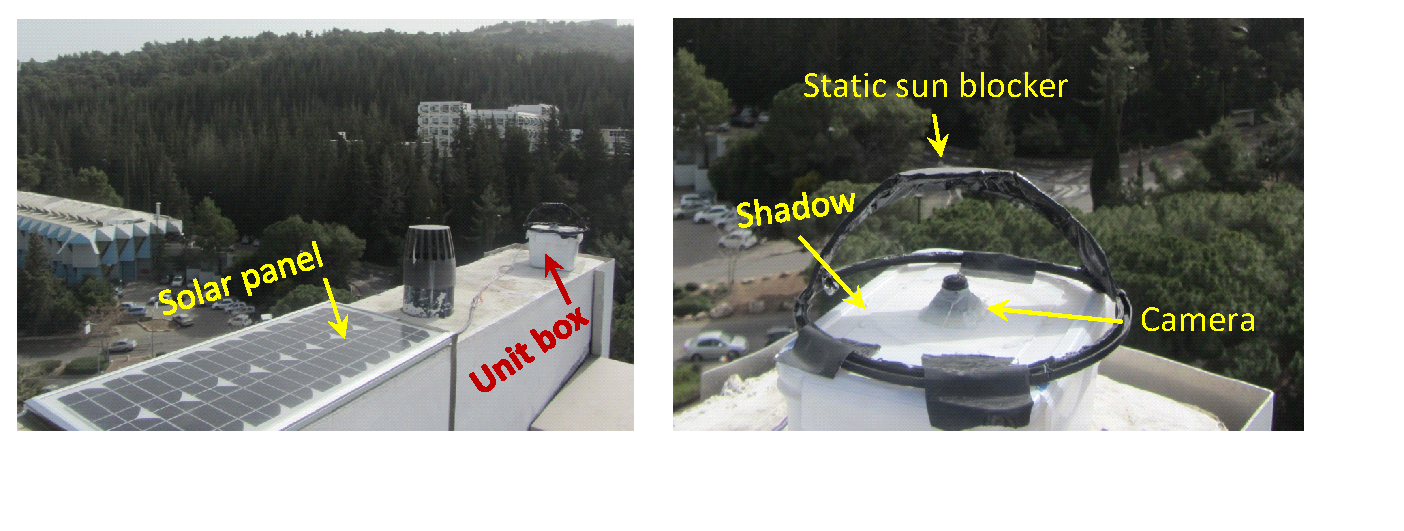
\includegraphics[width=0.6\linewidth]{figures/system.eps}
%\end{center}
%   \vspace{-0.6cm}
%   \caption{A unit (network-node) on a rooftop in a hilly area. It is based on a Raspberry-Pi camera
%   and uses solar energy. Its fisheye lens is shadowed here by a mounted  static Sun-blocker.
%   }
%\label{fig:system}
%\end{figure}
\begin{figure}[t!]
\begin{center}
   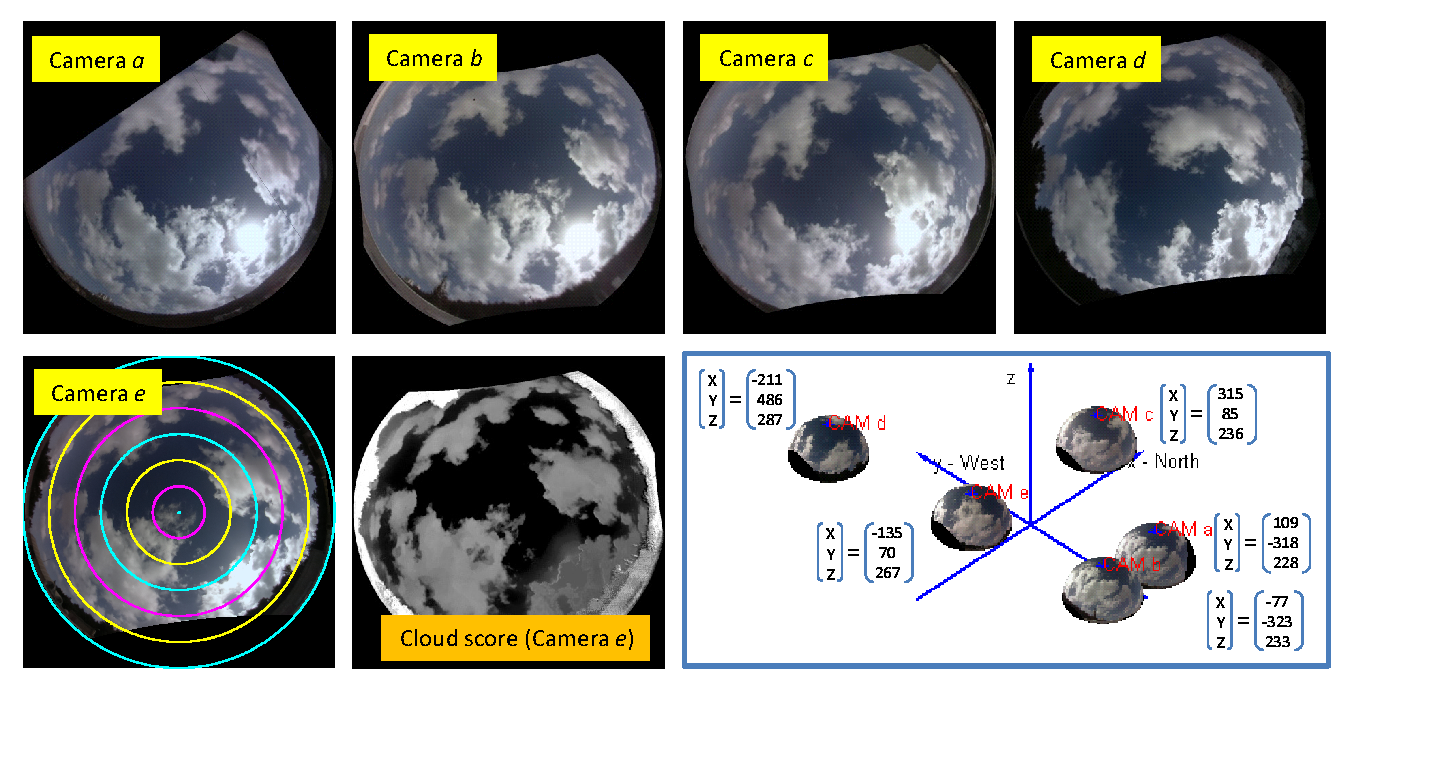
\includegraphics[width=1\linewidth]{figures/scene_d.eps}
\end{center}
   \vspace{-1.2cm}
   \caption{Images taken simultaneously by a 5-node network. They are geometrically aligned to the zenith and north, and resampled to {\em polar azimuthal equidistant} projection in this global system. Equidistant zenith angle circles are overlayed on $\tilde I_t[{\bf l}_e,{\bm \theta}]$ (camera $e$). Each camera has dead-regions, since the lens-axis had only been roughly centered on the tiny DIY boards.
   Corresponding to the frame in camera $e$, a {\em cloud score} map (Eq.~\ref{eq:sr}) has high values in cloud-pixels, diminishing outside them. [Bottom-right] The 3D setup of the experimental network. It is laterally spread over several hundreds of meters, on rooftops at somewhat different heights.}
\label{fig:photomotion}
\end{figure}



%%%%%%%%%%%%%%%%%%%%%%%%%%%%%%%%%%%%%%%%%%%%%%%%%%%%%%%%%%%%%%
\section{Inter-camera Relative Radiometric Self-Calibration}
\label{sec:mutiradio}

%
%%%%%%%%%%%%%%%%%%%%%%%%%%%%%%%%%%%%%%%%%%%%%%%%%%%%%%%%%%%%%%%
%\subsection*{The Experimental Setup}
%\label{sec:system}
%

Consider a {\em fixed} view direction ${\bm \theta}$ observed by several cameras.
%, e.g., $c$ and $c'$.
The values $\{\tilde I_t[{\bf l}_c,{\bm \theta}]\}_c$ correspond to readouts of parallel rays, back-projected from all cameras in the network. The values in this set generally differ from each other, e.g.,
 $\tilde I_t[{\bf l}_c,{\bm \theta}]\neq \tilde I_t[{\bf l}_{c'},{\bm \theta}]$. There are two causes for this difference:\\
 {\tt 1}.~ Different camera locations mean different observed objects. Momentarily, camera $c$ may observe a cloud while $c'$ observes a clear sky, or vice versa. Camera $c'$ may momentarily observe a somewhat denser haze volume than $c$, or vice versa. \\
 {\tt 2}.~ Slight inter-camera radiometric inconsistencies, which we need to estimate.\\
 Cause {\tt 1} is usually dominant. We need to overcome it, in order to analyze cause {\tt 2}.

The assumption we make is of {\em regional stationarity}. In a region containing the cameras, the chance of a cloud, clear sky, or haziness affecting $\tilde I_t[{\bf l}_c,{\bm \theta}]$ is {\em independent} of $c$. Thus, inter-camera image variations due to atmospheric conditions are {\em random and unbiased}. Per camera $c$ and view angle ${\bm \theta}$, bias is due to cause ({\tt 2}). We easily detect and characterize the bias by capturing {\em statistics over time}.
\begin{figure}[t!]
  \begin{center}
    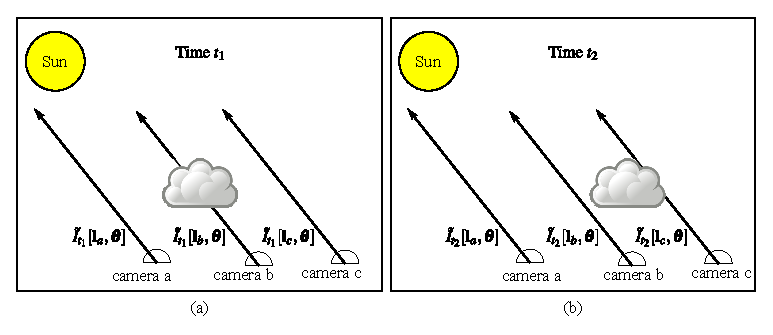
\includegraphics[width=\linewidth]{figures/regional_stationarity.eps}
  \end{center}
  \vspace{-0.6cm}
  \caption{[a] and [b] show the same camera network at times $t_1$ and
    $t_2$ respectively. The "regional stationarity"
concept could be explained in more detail, objects at optical infinity (i.e. background
    sky) should have the same color for a common viewing angle ${\bm
      \theta}$ (e.g. $\tilde I_{t_1}[{\bf l}_a,{\bm \theta}]$ and
    $I_{t_1}[{\bf l}_c,{\bm \theta}]$), whereas objects that are
    closer (clouds) would show a parallax and therefore result in
    pixel differences (e.g. $\tilde I_{t_1}[{\bf l}_b,{\bm \theta}]$
    and $I_{t_1}[{\bf l}_c,{\bm \theta}]$). We can exclude the second
    case using the statistical and camera independence of clouds
    (e.g. $\tilde I_{t_1}[{\bf l}_b,{\bm \theta}]$ vs. $\tilde
    I_{t_2}[{\bf l}_b,{\bm \theta}]$). Any residual bias can be
    attributed to the slight inter-camera radiometric inconsistencies
    that we would like to estimate.  }
  \label{fig:calibration}
\end{figure}
Consider, for example, Fig.~\ref{fig:calibration}a. It shows radiometric inconsistency between cameras $a$ and $b$. The figure then shows a scatter-plot of
$\tilde I_t[{\bf l}_a,{\bm \theta}]$ vs.~$\tilde I_t[{\bf l}_{b},{\bm \theta}]$, $\forall t,{\bm \theta}$, for the red-channel.
\begin{figure}[t!]
\begin{center}
   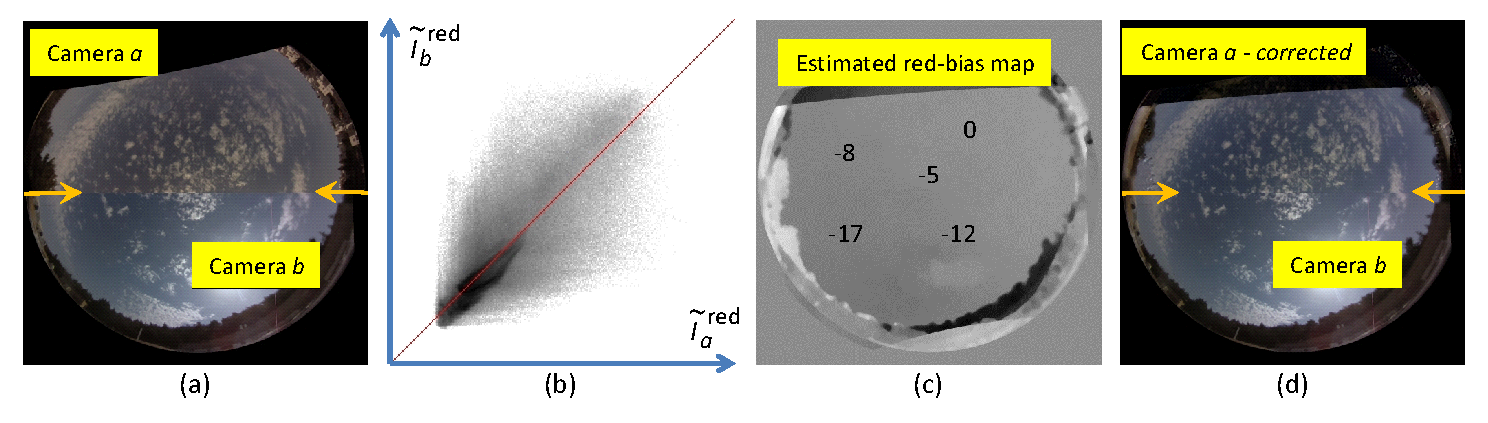
\includegraphics[width=\linewidth]{figures/bias4.eps}
\end{center}
   \vspace{-0.6cm}
   \caption{[a] Splitting the field of view to upper/lower halves, to pixels corresponding
   respectively to either $\tilde I_t[{\bf l}_a,{\bm \theta}]$  or $\tilde I_t[{\bf l}_{b},{\bm \theta}]$. In the line between the marked arrows, Radiometric inconsistency shows-up as a seam across which colors slightly change ({\bf please view on a color computer screen}). [b] Scatter-plot of
   $\tilde I_t[{\bf l}_a,{\bm \theta}]$ vs.~$\tilde I_t[{\bf l}_{b},{\bm \theta}]$, $~\forall t,{\bm \theta}$, red-channel. [c] The estimated offset map ${\hat o}_{b-a}({\bm \theta})$, red channel. It is derived based on a set of images taken during several hours.
   [d] Splitting the field of view in half, to {\em corrected} pixels from either
   $\hat I_t[{\bf l}_a,{\bm \theta}]$  or $\hat I_t[{\bf l}_{b},{\bm \theta}]$: inconsistencies in the line between the marked arrows are greatly
   diminished.
   }
\label{fig:calibration}
\end{figure}
From this scatter plot and those of the other color channels, we hypothesized that camera $a$ has a slight offset, particularly in the red channel, relative to camera $b$. We thus estimated, per color channel, the map of radiometric offset (across pixels, or ray-directions). A temporal median was used.
\begin{equation}
 {\hat o}_{b-a}({\bm \theta})=
  {\rm median}_{t} \{\tilde I_t[{\bf l}_b,{\bm \theta}]-I_t[{\bf l}_a,{\bm \theta}]\}.
 \label{eq:hato}
\end{equation}
The map ${\hat o}_{b-a}({\bm \theta})$ was then spatially smoothed and used to correct $\tilde I_t[{\bf l}_a,{\bm \theta}]$. As shown in Fig.~\ref{fig:calibration}, the results have much better inter-camera consistency. This is apparent in images taken throughout that day. A similar process was applied to other cameras, but they had negligible radiometric offsets with respect to camera $b$. Later, it was obtained that cause for the severe Radiometric deviations of camera $a$ was a red led located near the sensor.
Overall, it's important to note that the Radiometric calibration scheme described here does not claim to perform global Radiometric calibration(which can be performed a-priori on each camera), but aims at resolving relative Radiometric deviations caused in-situ by dirt or ...

The process was then repeated to detect slight local variations of gain (vignetting). Suppose there is no offset. In analogy to Eq.~(\ref{eq:hato}), the gain in $b$ is higher than in $a$ by a factor
\begin{equation}
 {\hat M}_{b/a}({\bm \theta})=
  {\rm median}_{t} \{\tilde I_t[{\bf l}_b,{\bm \theta}]/I_t[{\bf l}_a,{\bm \theta}]\}
 \label{eq:hatm}
\end{equation}
Under this scheme all the cameras in the network are radiometrically aligned to a single master camera.
After radiometric corrections, the light-field samples are denoted $\hat I_t[{\bf l}_b,{\bm \theta}]$.


%%%%%%%%%%%%%%%%%%%%%%%%%%%%%%%%%%%%%%%%%%%%%%%%%%%%%%%%%%%%%%
\section{Network-assisted Background Estimation}
\label{sec:background}

It is often helpful to characterize the background, as motivated by change-detection computer vision algorithms. In monocular settings, such algorithms use temporal filtering to characterize the background\footnote{Physical sky appearance models~\cite{hosek2012analytic} require several atmospheric parameters that are unknown in our case, e.g. the aerosol distribution}: foreground dynamic objects are at {\em different locations at different times} and are thus pruned. In our case this translates to stating that a cloud in
$\tilde I_t[{\bf l}_c,{\bm \theta}]$ is often not in
$\tilde I_{t'}[{\bf l}_c,{\bm \theta}]$, when $t'\neq t$. However, if clouds move slowly, while illumination gradually changes, temporal filtering may be insufficient. This is illustrated in Fig.~\ref{fig:sky}.

A light-field network enhances this principle, with more effective pruning-per-time. Here we demonstrate this idea by suggesting a simple yet effective background estimation method. Any other monocular state-of-the-art method of background estimation can be enhanced using the network approach. After calibration, {\em simultaneous} images captured by {\em different camera nodes} are different from each other. Thus, change of viewpoint has an effect similar to change in time: a cloud in
$\tilde I_t[{\bf l}_c,{\bm \theta}]$ is often not in $\tilde I_t[{\bf l}_{c'},{\bm \theta}]$. This principle relies on the {\em regional stationarity} mentioned above. Consequently, background sky values are obtained by data filtering over both time and viewpoint.

In broad daylight, clouds are brighter than the blue sky. Hence, as an example, an estimator for the sky background can be:
\begin{equation}
 {\rm SKY}({\bm \theta})= \arg\min_{t,c} \tilde I_t[{\bf l}_c,{\bm \theta}]
 \label{eq:SKY}
\end{equation}
where $t\in[1\ldots N^{\rm frames}]$ and $c\in[1\ldots N^{\rm views}]$.
This is illustrated in Fig.~\ref{fig:sky}.
\begin{figure}[t!]
\begin{center}
   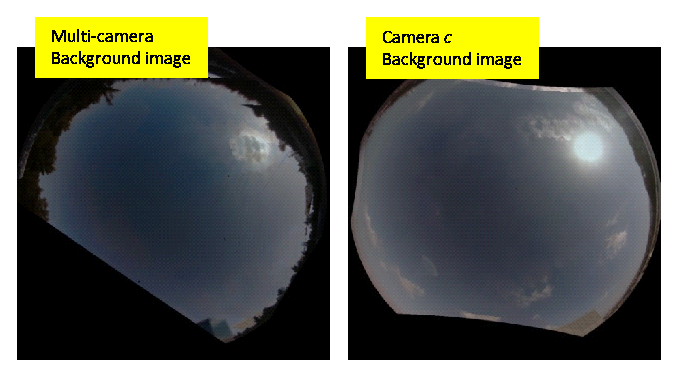
\includegraphics[width=0.5\linewidth]{figures/Background.eps}
\end{center}
   \vspace{-0.6cm}
   \caption{[Left] Estimation of the sky background, using Eq.~(\ref{eq:SKY}) based on five temporal
   instances and five viewpoints. [Right] Estimation of the sky background, using five temporal
   instances, but just a single viewpoint, resulting in more residual clouds.}
\label{fig:sky}
\end{figure}


%%%%%%%%%%%%%%%%%%%%%%%%%%%%%%%%%%%%%%%%%%%%%%%%%%%%%%%%%%%%%%
\section{Bypassing the Sun through a Camera Network}
\label{sec:mutiSun}

As Sec.~\ref{sec:Signelflare} explains, in existing full sky-imagers, effects of direct sunlight are often mitigated by a small dynamic sun-blocker, which complicates the system and its cost, while having a blind-region. The network offers a different solution, which can be radical, yet simple. On each camera, the sun-blocker is {\em static}, and has no moving part. The blocker can be large, covering the entire range of directions the Sun may occupy during the year or part of it. In this configuration, each camera unit has a large blind area (See Fig.~\ref{fig:blindspot}). Nevertheless, the entire {\em network has no blind spot}, when viewing the atmosphere. This remarkable property is a result of network-redundancy, as we explain.
\begin{figure}[t!]
\begin{center}
   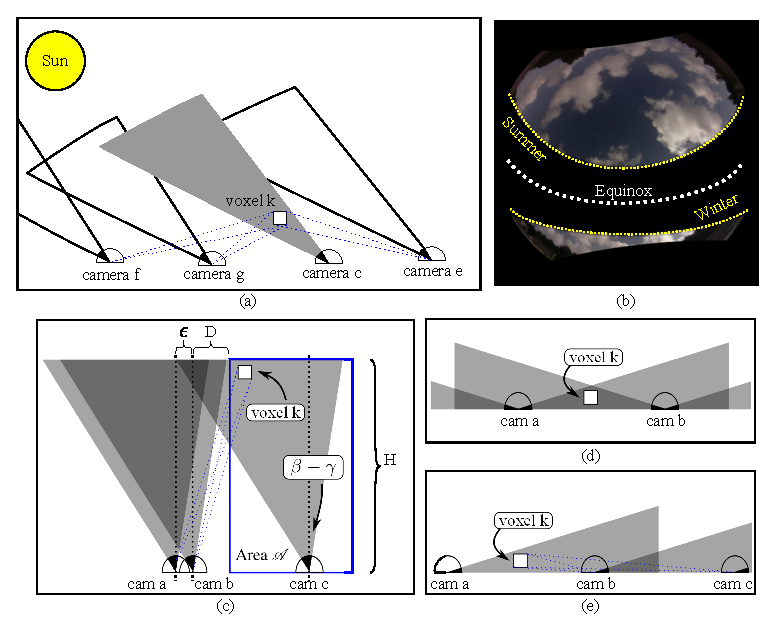
\includegraphics[width=0.8\linewidth]{figures/sun_blocks2.eps}
\end{center}
   \vspace{-0.6cm}
   \caption{[a] Camera $c$ has a blind-region, covering Sun directions at ${\bf l}_c$. The blind region corresponds to set $\Gamma_c$ of atmospheric voxels not sensed by by camera $c$. The network as a whole still has coverage of voxels $k\in\Gamma_c$, as they are observed by cameras $e,f,g$.
   [b] Simulation of a whole sky image (polar azimuthal equidistant projection), blocking
   all solar directions during the year, at a mid-latitude.
   [c] In the topics, the network must have nodes at distance $D$ outside surveyed area ${\cal A}$, if ${\cal A}$ is narrow.  The distance D depends on the latitude $\gamma$, while
   $\beta\approx23.5^o$.
   [d] In the arctic, the blind region is adjacent to the horizon, in all azimuth angles. Fixed blocking of the Sun over $360^o$  blocks low-altitude voxel $k$. [e] Arctic cameras fitted with a fixed north-facing sun blocker create a network   that operates 12 hours a day. An adjacent camera at each node has a fixed south-facing sun blocker, for imaging during complementing hours.
   %For tropic cameras, the blind region dissects the field from east to west through the Zenith. In the arctic, the blind region is adjacent to the horizon.
   }
\label{fig:blindspot}
\end{figure}


A static year-round sun blocker on camera $c$ permanently obstructs a set $\Gamma_c$ of atmospheric voxels. These voxels, however, are generally visible at several other cameras, e.g., those indexed $e,f,g$ in Fig.~\ref{fig:blindspot}. Consequently, a sufficiently wide network has no 3D blind spot, despite permanent sun-blocking. Voxels that are not obstructed from any camera have more viewpoints to constrain their content, than voxels in $\Gamma_c$.

We now quantify the implication of this approach to the network extent, referring to the northern hemisphere without loss of generality.
Nearly all weather phenomena are under the tropopause, whose altitude $H$ above sea level is typically 17km at the equator, and decreasing with latitude. The solar seasonal angle amplitude is $\beta\approx23.5^o$. At latitude $\gamma$, thus, a permanent sun blocker spans zenith angles in the range $\gamma\pm\beta$. Earth is divided here to three region classes:\\
  ${\bf \bullet}$ In the tropics, the sky directly above a camera is blocked. Consider
  a small tropical area ${\cal A}$, e.g., 1km wide, whose sky needs to be monitored. According to Fig.~\ref{fig:blindspot}c, ${\cal A}$ can efficiently be observed without
  a blind spot by cameras to its {\em south}. The network needs to have camera units extending to distance  $D=H\tan(\beta-\gamma)+\epsilon$ from ${\cal A}$, where $\epsilon$ is a small distance, sufficient for triangulation at $H$. At the equator $D\approx7.4$km.
  It can also be shown that if ${\cal A}$ is wider than $2H[\tan(\beta-\gamma)+\tan(\beta+\gamma)]$, the network can observe and triangulate all the sky right above it.\\
${\bf \bullet}$  As latitude increases towards the tropic circles, $D$ decreases to zero. Thus the network can observe and triangulate all the sky right above it, anywhere outside the tropics, in the mid-latitudes.\\
  ${\bf \bullet}$ In the arctic and antarctic summer, the Sun can appear in all azimuth angles over the day. A single 24-hour fixed sun-blocker blocks the horizon. So as shown in Fig.~\ref{fig:blindspot}d, voxel $k$ is not observed. One solution would be to mount two cameras, side by side, in each network node. Each camera in a node has a fixed sun blocker effective covering half of the azimuth angles. One camera operates in the {\em polar daytime} (local 6AM to 6PM), as it has a south-oriented fixed blocker. The other camera operates in the complementing time (Fig.~\ref{fig:blindspot}e), having a north-oriented fixed blocker. This way, the network never has a blind spot.


%%%%%%%%%%%%%%%%%%%%%%%%%%%%%%%%%%%%%%%%%%%%%%%%%%%%%%%%%%%%%%
\section{3D Clouds by a Camera Network}
\label{sec:3Dc}

Network-based acquisition and the processes described above, yield a calibrated sampled light-field of the sky. Using this light-field, one application is to estimate the 3D cloud structure above the network domain, and beyond. This is done by the following steps:~ %({\tt A})~Estimate the background;~
({\tt A})~Per time $t$, give a {\rm cloud score} $s$  to each ray $[{\bf l}_c,{\bm \theta}]$, as we explain below.~({\tt B})~Perform a fuzzy version of space carving~\cite{Kutulakos2000,Ihrke2004} (reminiscent of back-projection in tomography).

We first describe a simple yet effective method to implement ({\tt B}).  The set of all sampled light-field rays is ${\cal R}$, where
\mbox{$|{\cal R}|=N^{\rm rays}$}. A ray is indexed by $r$, and it corresponds to a specific $[{\bf l}_c,{\bm \theta}]$. Voxel $k$ projects to a subset of the rays $\rho_k\subset{\cal R}$,
that reach $\nu_k$ viewpoints. Suppose a ray $r\in{\cal R}$ has a cloud-score $s(r)\in[0,1]$, where $s=0$ means there is definitely no cloud on the ray, while $s=1$ means there is confidently a cloud there. Per voxel $k$, define a back-projected score
\begin{equation}
 B_k= \left[ \prod_{r\in\rho_k} s(r)\right]^{1/\rho_k}
 \;\; ~~{\rm if}~~ \nu_k\geq 2
  \;.
 \label{eq:Bk}
\end{equation}
The back-projected score of voxel $k$ is null, if $k$ is not observed by at least two viewpoints. This score is null also if $s(r)=0$ for any $r\in\rho_k$. If all $r\in\rho_k$ have same score $s$, then $B_k=s$. Equation~(\ref{eq:Bk}) carves-out voxels that contradict support for clouds.

Different cloud regions have signature appearances. Ignoring this would wrongly allow matching of, say, a darker cloud-bottom to a bright sun-lit side of a cloud, or a smooth cloud region to a textured one. Thus, photometric and appearance consistency across viewpoints is incorporated (the photo-hull concept in space-carving~\cite{Kutulakos2000}). Clouds are diffuse, cooperating with this requirement.
From the images, a feature vector ${\bf v}(r,t)$ is extracted for any measured ray $r$.
We used SIFT descriptors~\cite{lowe2004distinctive} and the radiance in each color channel. Element $q$ of ${\bf v}(r,t)$ is $v_q(r,t)$. The values of this element, for all rays that intersect voxel $k$, is \mbox{${\cal V}_q(k,t)\equiv\{v_q(r,t)\}_{r\in\rho_k}$}.
Across viewpoints, the measured variance in this set is
${\rm VAR}[{\cal V}_q(k,t)]$. Define an appearance consistency score~\cite{Supp2014} as
\begin{equation}
 P_k= \exp\left(
         -\Sigma_q\{[{\cal V}_q(k,t)]\}/\sigma^2
         \right)
  \;,
 \label{eq:Dist}
\end{equation}
where $\sigma^2$ is a scale parameter. Overall, the total cloud-score of a voxel is $T_k=B_kP_k$.

The resulting 3D field $\{T_k\}$ is a volumetric estimate of cloud occupancy. It is biased to yield clouds larger than they really are: high-altitude voxels occluded by the cloud-base from all viewpoints are interpreted as being cloudy, since for them $T_k$ is high. This is a realization of a basic ambiguity: if a voxel is occluded from all viewpoints, then there is no way of telling if it is cloudy or not, unless auxiliary or prior knowledge is available. Incorporating a visibility prior favors smaller clouds that explain the data. If voxel $k$ is completely occluded by other cloudy voxels, then it is pruned (carved) out. Voxel $k$ can only maintain its $T_k$ if there are at least two camera viewpoints from which $k$ is not occluded by other clouded voxels. This pruning is achieved by sweeping~\cite{Kutulakos2000} the field $\{T_k\}$ iteratively. The pruned 3D cloud occupancy field is denoted $\{\tilde T_k\}$. We can maintain the non-binary (fuzzy) nature or $\{\tilde T_k\}$. This way, it possesses the inherent semi-transparency and subtle ambiguity of clouds.

%%%%%%%%%%%%%%%%%%%%%%%%%%%%%%%%%%%%%%%%%%%%%%%%%%%%%%%%%%%%%%
\subsection*{Basic cloud score}
\label{sec:cloudscore}


For a basic cloud score (step {\tt A}), there are various functions in the literature. We considered several of them, including using the background derived in Sec.~\ref{sec:background}. There is certainly room for increased sophistication, including sky modeling and machine learning, but we choose to stick with a simple measure. The ratio of image readout at the red/blue color channels, $\tilde I^{\rm red}/\tilde I^{\rm blue}$, is widely used in the literature~\cite{Yamashita2004,Seiz2002}. Overall, we found it to be an effective feature in broad daylight: clouds are grey (unit red-blue ratio), and the cloudless sky is significantly biased to blue
(below $\approx 0.8$ red-blue ratio). Thus, for demonstrations in this paper,
the cloud-score we used per ray (pixel) is
\begin{equation}
 s(r)=\left\{
      \begin{array}{ll}
      \frac{6 [\tilde I^{\rm red}(r)/\tilde I^{\rm blue}(r)-0.8]}
           {0.2+\tilde I^{\rm red}(r)/\tilde I^{\rm blue}(r)}
      & ~~~~{\rm if}~ \tilde I^{\rm red}(r)/\tilde I^{\rm blue}(r)>0.8 \\
      0
      & ~~~~{\rm otherwise}
      \end{array}
      \right.
  \;.
 \label{eq:sr}
\end{equation}
Here $s\in[0,1]$, where either bound is achieved at gray clouds or blue sky, repectively. An example of applying this operator on an image is shown in Fig.~\ref{fig:photomotion}.



%%%%%%%%%%%%%%%%%%%%%%%%%%%%%%%%%%%%%%%%%%%%%%%%%%%%%%%%%%%%%%
\subsection*{Simulations}
\label{sec:simulation}

Quantitative assessments used atmospheric-science gold standard simulators.
An atmosphere over $8\times8{\rm km}$  was produced using off-the-shelf large eddy simulation (LES), creating clouds between heights of $500{\rm m}$ to $1500{\rm m}$.
Lighting conditions were consistent with Copenhagen (unrelated to the anonymous authors).
Radiative transfer using the discrete ordinate spherical-harmonic method (SHDOM)~\cite{Evans1998} rendered images taken by 100 cameras placed in a $2.5\times 2.5{\rm km}^2$ domain. Recovery simulations used random subsets
of the network, where the whole network is either with or without
a sun blocker. In the LES, a voxel is occupied by cloud if its water-mass parameter is not null. In the recovery, voxel $k$ is classified as cloud if $T_k>0.01$.
We measured the classification error rate, across all voxels.
% Note that the LES example
%details the  water particle distribution and therefore $B$ is calculated
%as the voxels where the water content equals are surpasses some threshold.
%The threshold we used was half the maximal water content in the example.
%Due to this method we don't expect to achieve perfect reconstruction.
The results are plotted in Fig.~\ref{fig:simulations}.  As expected of space carving,
results improve fast from 2 to 10 cameras. Even when a sun blocker is applied,
the algorithm is able to reconstruct the cloud formation. As expected,
more cameras are needed in order to compensate for the limited view of
each camera.
\begin{figure}
  \begin{center}
    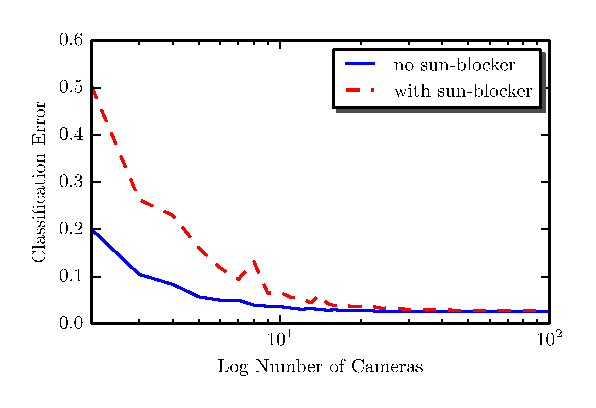
\includegraphics{figures/simulations.eps}
    \caption{Classification error rate as a function of the number of
    cameras. [Solid Blue] Without sun blocker. [Dashed Red] With sun blocker.
    Fluctuations are within the random sampling standard deviation.}
    \label{fig:simulations}
  \end{center}
\end{figure}


%%%%%%%%%%%%%%%%%%%%%%%%%%%%%%%%%%%%%%%%%%%%%%%%%%%%%%%%%%%%%%
\subsection*{Cloud Reconstruction Experiment}
\label{sec:results}

We applied the approach on various captured scenes\footnote{Sun blocker was not used here due to the fact that Saturation and Blooming effects do not impair cloud reconstruction efforts.}. One scene had cumulus clouds, similar to those seen in Fig.~\ref{fig:photomotion}.
%
%
%Fig.~\ref{fig:cu} shows sample frames of one scene, having cumulus clouds.
%\begin{figure}[t!]
%\begin{center}
%   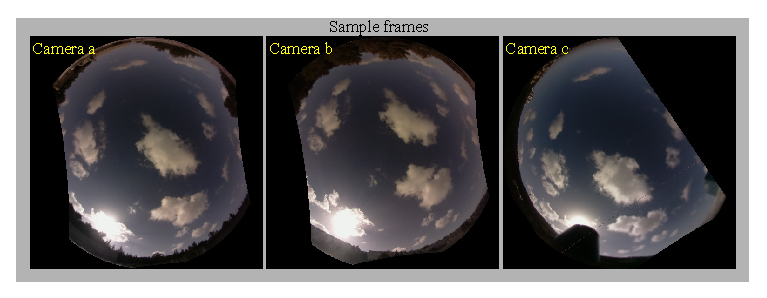
\includegraphics[width=1\linewidth]{figures/projection.eps}
%\end{center}
%   \vspace{-0.6cm}
%   \caption{Cumulus clouds. Frames taken from multiple views, aligned and  shown in polar azimuthal equidistant projection.
%   }
%\label{fig:cu}
%\end{figure}
Cross-sections of the recovered 3D cloud-occupancy field $\{\tilde T_k\}$ are shown in Fig.~\ref{fig:projection}. The lateral domain of the clouds is much larger than the camera network.
\begin{figure}[t!]
\begin{center}
   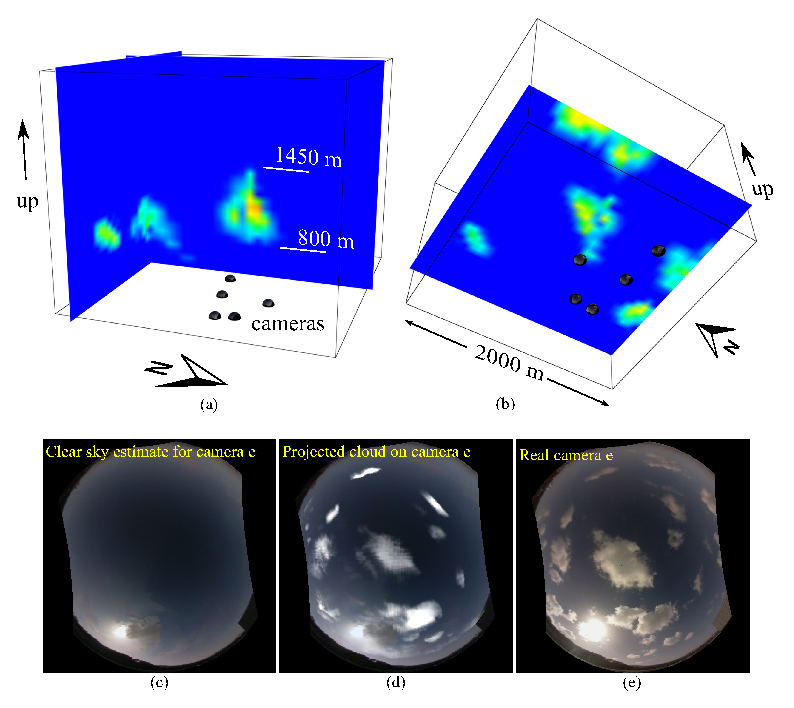
\includegraphics[width=1\linewidth]{figures/clouds_reconstructions.eps}
\end{center}
   \vspace{-0.6cm}
   \caption{3D cumulus cloud recovery results. (a,b) Cross-sections of the recovered cloud-occupancy field $\{\tilde T_k\}$. Note how the domain of the clouds is much larger than the camera network. Cloud
   altitude is above sea-level. (c) Estimated sky-background image.  Based on four viewpoints (indexed $a,b,c,d$), the 3D volumetric cloud-occupancy field $\{\tilde T_k\}$ was derived. The field $\{\tilde T_k\}$ was projected to viewpoint $e$, and overlayed on the estimated sky-background image. The resulting synthetic cloud-score image $J[{\bf l}_e,{\bm \theta}]$ is shown in (d). This can be compared to the real captured image $\hat I_t[{\bf l}_e,{\bm \theta}]$, shown in (e).}
\label{fig:projection}
\end{figure}
Accounting for the altitude of the cameras above sea-level, the clouds mainly reside between 800m to 1450m above Sea-level. We used two indicators to validate the results. First, there are worldwide balloon-based radiosonde measurements including quantitative vertical humidity profiles. The radiosonde nearest to our network is 88km away, on a similar coastal strip, and used by forecasters for our location. It indicated a layer of high humidity that can yield clouds in the range $[770,1881]$m above sea-level, consistent with our clouds.

Second, we cross-validated 3D recovery {\em with missing field of view}. We used four cameras (indexed $a,b,c,d$) out of five, for 3D estimation. Camera $e$ was ignored. Then, we projected the estimated 3D cloud distribution into viewpoint $e$, and compared to the ground truth. The rendered image is as follows. {\em Ray casting}~\cite{Levoy1990} of  field $\{\tilde T_k\}$ is performed on a ray corresponding to
$[{\bf l}_e,{\bm \theta}]$. Ray-casting aggregates $\{\tilde T_k\}$ on all voxels intersected by the ray. The result is a cloud-score image $w[{\bf l}_e,{\bm \theta}]$.
To visualize $w[{\bf l}_e,{\bm \theta}]$, we used it as $\alpha$-map to the estimated sky-background image (Eq.~\ref{eq:SKY}). The alpha-map is
\begin{equation}
 \alpha[{\bf l}_e,{\bm \theta}]=\left\{
      \begin{array}{ll}
      2w[{\bf l}_e,{\bm \theta}]
      & ~~~~{\rm if}~ 2w[{\bf l}_e,{\bm \theta}]<1 \\
      1
      & ~~~~{\rm otherwise}
      \end{array}
      \right.
  \;.
 \label{eq:alpha}
\end{equation}
The rendered image is then
%\begin{equation}
 $J[{\bf l}_e,{\bm \theta}]=
 \alpha[{\bf l}_e,{\bm \theta}]+(1-\alpha[{\bf l}_e,{\bm \theta}]){\rm SKY}({\bm \theta})$.~
%  \;.
% \label{eq:alpha}
%\end{equation}
This image does not pretend to properly render clouds in their true shades and effect on the sky. It simply served to visualize the result, as shown in Fig.~\ref{fig:projection}d. It can be compared to the true corresponding image $\hat I_t[{\bf l}_e,{\bm \theta}]$, in Fig.~\ref{fig:projection}e.
This rendering relies on the redundancy of the network. Even if a viewpoint is blocked, much of its information can be derived using other viewpoints compounded with 3D recovery. This is consistent with the proposed approach for handling static partial blocking of viewfields. See more results in ~\cite{Supp2014}.

Another scene had a layer of alto-cumulus clouds. Figure~\ref{fig:alto} shows sample frames from this scene, and cross-sections of the recovered 3D cloud-occupancy field $\{\tilde T_k\}$.
\begin{figure}[t!]
\begin{center}
   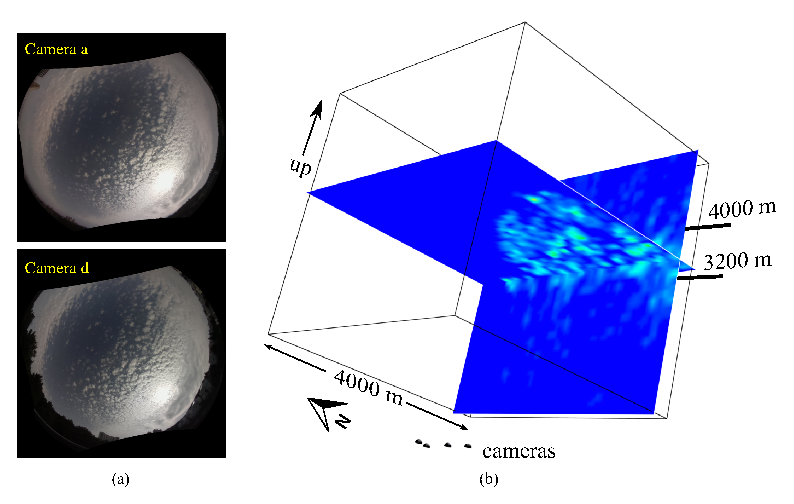
\includegraphics[width=1\linewidth]{figures/altos.eps}
\end{center}
   \vspace{-0.6cm}
   \caption{3D altocumulus cloud recovery results. (a,b) Sample frames.
   (c,d)  Cross-sections of the recovered cloud-occupancy field $\{\tilde T_k\}$. Cloud
   altitude is above sea-level.}
\label{fig:alto}
\end{figure}
Accounting for the altitude of the cameras above sea-level, these estimated clouds mainly reside on a horizontal layer 3450m above sea-level, and the layer is about a kilometer thick. This time, the radiosonde readout indicated a layer of high humidity that can yield clouds in height range $[3072,4180]$m above sea-level. This is in strong agreement with our results.





%The pose can be self-calibrated using multiview geometry, particularly {\em structure from motion} (SfM), which has been extensively developed~\cite{birkbeck,cremers,matousek,pollefeys,ruf,woodford} by the computer vision community. A preliminary result is shown in Fig.~\ref{fig:clouds2}, obtained by the Israeli group.
%


%%%%%%%%%%%%%%%%%%%%%%%%%%%%%%%%%%%%%%%%%%%%%%%%%%%%%%%%%%%%%%
\section{Discussion}
\label{sec:discuss}

Scaling light-field imaging hugely to sense the sky, would use  a large network of camera nodes, each having a hemispherical field of view, deployed over a wide area. Such a network can reach anywhere wireless communication exists, and in principle can be a continent-wide light-field system. This sensing approach offers significant advantages over existing technologies (experimental and operational) of atmospheric sensing, particularly  3D imaging, and doing so in high spatio-temporal resolution. This sensing approach poses new questions for computer vision and computational photography. These include network-based extensions to monocular tasks including network-based radiometric calibration and background estimation. Network redundancy offers the ability of by-passing saturation or blind spots, as those created by the sun, without moving parts.

To enable a massive network, each node should have very low-cost. To demonstrate this can work, we built the units in our experimental small-network using very basic components and coarse alignment tolerances. In a long term, mass producing consistent units would ensure proper alignment performance (non dead-regions) and operational robustness over long periods. Still, this concept opens the door to more interesting research. In the direction of the sun blocker, a diffraction grating can disperse direct sunlight (currently blocked) or skylight, to measure its spectrum. This principle is already used by Aeronet~\cite{Holben1998} to characterize aerosols. Night-time operation is another interesting challenge: if a known planet and star appears missing on ray $r$, this indicated a cloud on $r$. Furthermore, such a light-field system can be used for studying bird life, in 3D time-lapses.






%===========================================================
\bibliographystyle{splncs}
\bibliography{cloudsbib}

%this would normally be the end of your paper, but you may also have an appendix
%within the given limit of number of pages
\end{document}
